%\lstset{breakatwhitespace=true,breaklines=true}
\section{ISTL and PDELab Backends}
\label{sec:pdelab-backends}


\subsection{The Iterative Solver Template Library}
\label{sec:iter-solv-templ}

\subsubsection{Block Structure in FE Matrices}
\label{sec:motivation}
\begin{frame} \frametitle{The Iterative Template Library}
  \framesubtitle{PDE Systems}
  \begin{block}{}
      We have several unknowns and therefore several grid functions
      when dealing with PDE Systems.
      For the simple case that each function has the same structure we
      can use the following special ordering and blocking approaches:
  \begin{itemize}
  \item Equation-wise blocking: All degrees of freedom associated with
    the same unknown are blocked together.
  \item Point-wise blocking: All degrees of freedom associated with
    the same point (or element) are blocked together.
  \item No blocking is used.
  \end{itemize}
  \end{block}
  Currently the last two approaches are supported by PDELab with the
  ISTL backend.
\end{frame}
In the pictures below the degrees of freedom are visualized using
circles at the positions/entities they are associated with. Circles
with the same colour are blocked together. In the the entries in the
resulting matrix are dense and sparse matrices for the equation-wise
and point-wise blocking, respectively.
\begin{frame}
\frametitle{Some Examples for Block Structure}
\begin{block}{}
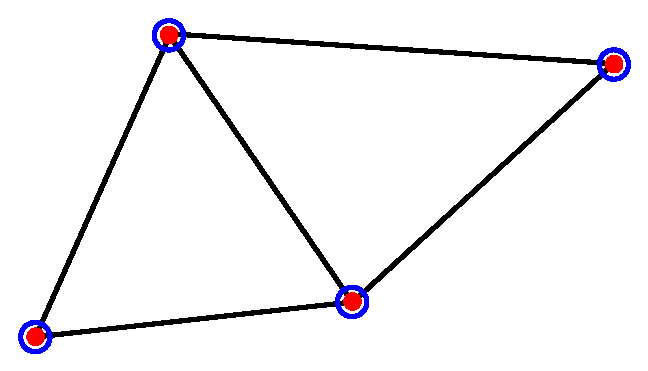
\includegraphics[width=0.48\textwidth]{./EPS/P1P1}\hfill
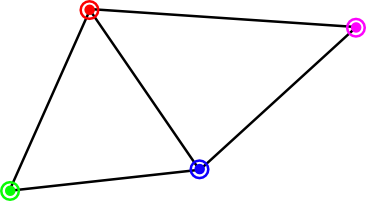
\includegraphics[width=0.48\textwidth]{./EPS/P1P1b}

\begin{minipage}{0.48\textwidth}
\centering $P_1\times P_1$ equation-wise
\end{minipage}
\begin{minipage}{0.48\textwidth}
\centering $P_1\times P_1$ point block
\end{minipage}

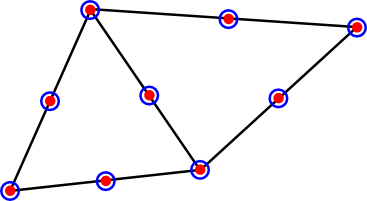
\includegraphics[width=0.48\textwidth]{./EPS/P2P2}\hfill
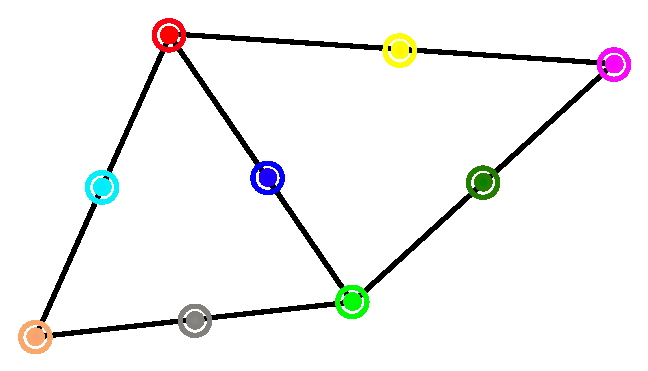
\includegraphics[width=0.48\textwidth]{./EPS/P2P2b}

\begin{minipage}{0.48\textwidth}
\centering $P_2\times P_2$ equation-wise
\end{minipage}
\begin{minipage}{0.48\textwidth}
\centering $P_2\times P_2$ point block
\end{minipage}
\end{block}
\end{frame}

\subsubsection{Matrix Vector Components}
\label{sec:matr-vect-comp}
\begin{frame}
\frametitle<presentation>{Matrix Vector Components in
  ISTL}
 \framesubtitle{Vector-Matrix Concept}
\begin{columns}[t]
\begin{column}{0.5\textwidth}
\begin{itemize}
\item Vector
\begin{itemize}
\item Is a one-dimensional container
\item Sequential access
\item Random access
\item Vector space operations: Addition, scaling
\item Scalar product
\item Various norms
\item Sizes
\end{itemize}
\end{itemize}
\end{column}
\pause
\begin{column}{0.5\textwidth}
\begin{itemize}
\item Matrix
\begin{itemize}
\item Is a two-dimensional container
\item Sequential access using iterators
\item Random access
\item Organization is row-wise
\item Mappings $y = y+Ax; y = y+A^Tx; y = y+A^Hx;$
\item Solve, inverse, left multiplication
\item Various norms
\item Sizes
\end{itemize}
\end{itemize}
\end{column}
\end{columns}
\end{frame}
\begin{frame}\frametitle{Recursive Construction}
  \begin{block}{Vector Space}
      \begin{itemize}
      \item Let $V_i$, $i=1, 2, \ldots,  n$, be a normed vector space of dimension
        $n_i$ with a
        scalar product, then the $n$-nary Cartesian product
      \item The vector space $V$
        \begin{equation*}
          V :=  V_1\times V_2 \times \ldots \times V_n = \{(\vec v_1, \vec v_2,
          \ldots, \vec v_n) | \vec v_1 \in V_1,
          \ldots, \vec v_n \in V_n\}
        \end{equation*}
        is again a normed vector space of dimension $\sum_{i=1}^n n_i$
        with the canonical norm and scalar product.
      \item Procedure can be applied recursively.
      \end{itemize}
  \end{block}\pause
  \begin{block}{Linear Mapping}
    \begin{itemize}
    \item  Linear map $A: V \mapsto
W$ from vector space $V$ to vector space $W$.
    \item Recursive construction follows immediately from the construction
    of the range and domain.
    \end{itemize}
  \end{block}
\end{frame}

\begin{frame} \frametitle{Vector Classes}
  \begin{block}{\lstinline!template<class K, int n> FieldVector<K,n>!}
    \begin{itemize}
    \item Represents vector space $V=K^n$
    \item Field \lstinline!K! may be any numeric type (e.g.
      \lstinline!double!, \lstinline!float!,
      \lstinline!complex<double>!)
    \end{itemize}
  \end{block}
  \begin{block}{\lstinline!template<class B> BlockVector<B>!}
    \begin{itemize}
  \item Represents vector space $V=B^n$.
  \item ``Block type'' \lstinline!B! has to implement the vector
    interface.
\end{itemize}
  \end{block}
  \begin{block}{\lstinline!template<class B> VariableBlockVector<B>!}
    \begin{itemize}
    \item Represents a vector space having a two-level
      block structure:
      $$V=B^{n_1}\times B^{n_2}\times\ldots \times B^{n_m}\,,$$
      \mode<article>{($m$ blocks with block $i=1,\ldots,m$ consisting of $n_i$ blocks
      given by the type \lstinline!B!.}
    \item More efficient than resembled by vector classes above.
      (interpretation as $V=B^N$,  $N={\sum_{i=1}^{m} n_i}$ possible!).
    \end{itemize}
  \end{block}
\end{frame}
\begin{frame} \frametitle{Matrix Classes}
  \begin{block}{\lstinline!template<class K, int n> FieldMatrix<K,n,m>!}
    \begin{itemize}
    \item Represents linear map $M: V_1 \to V_2$, with$V_1=K^n$ and
      $V_2=K^m$.
      \item Field \lstinline!K! may be any numeric type (e.g.
        \lstinline!double!, \lstinline!float!,
        \lstinline!complex<double>!)
    \end{itemize}
  \end{block}
  \begin{block}{ \lstinline!template<class B> BCRSMatrix<B>!}
    \begin{itemize}
    \item Sparse Matrix with block compressed row storage.
    \item ``Block type'' \lstinline!B! must implement the matrix interface.
    \end{itemize}
  \end{block}
  \begin{block}{\lstinline!template<class B> VariableBCRSMatrix<B>!}
    \begin{itemize}
    \item Sparse Matrix of dense Matrices with varying block size.
    \item Represents a linear map between two vector spaces having a two-level
block structure $V=B^{n_1}\times B^{n_2}\times\ldots \times B^{n_m}$
and $W=B^{m_1}\times B^{m_2}\times\ldots \times B^{m_k}$
    \end{itemize}
  \end{block}
%   \begin{block}{``Fusion Matrix'' (Martin Weiser, ZIB Berlin)}
%     \begin{itemize}
%     \item Dense Matrix of sparse Matrices.
%     \item Size of dense matrix known at compile time.
%     \item Suitable e.g for variable-based Stokes.
%     \end{itemize}
%   \end{block}
\end{frame}

\begin{frame}[fragile]
\frametitle{Block Structure in ISTL Matrices}
\begin{block}{}
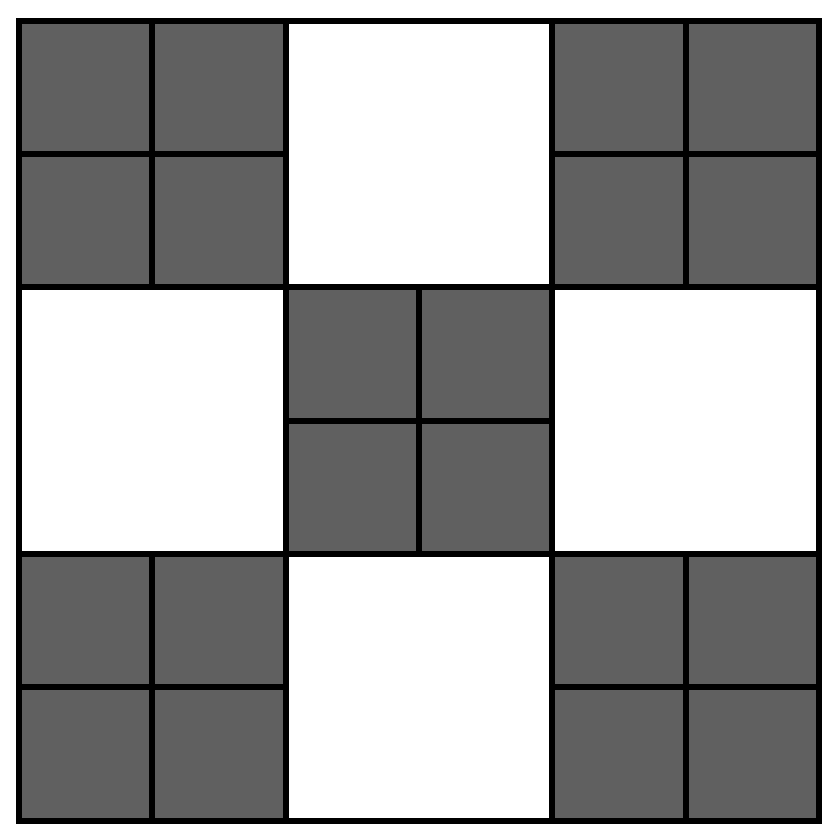
\includegraphics[width=0.3\textwidth]{./EPS/pointblockmatrix}\hfill
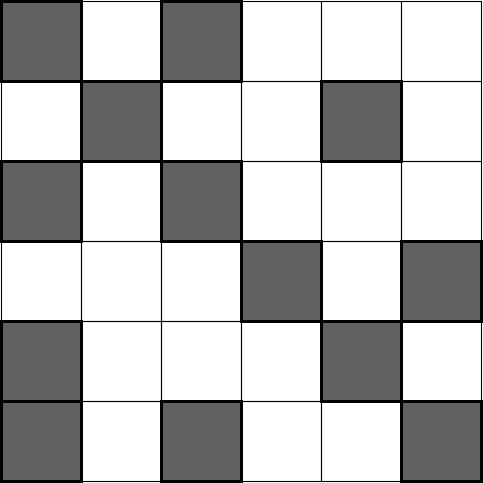
\includegraphics[width=0.3\textwidth]{./EPS/scalarmatrix}

\begin{minipage}{0.48\textwidth}
  \begin{itemize}
  \item  Point block matrix is a sparse matrix with small dense
blocks.
\item Realized by \lstinline[basicstyle=\tiny]!BCRSMatrix< FieldMatrix<E,2,2> >!.
  \end{itemize}
\end{minipage}
\begin{minipage}{0.48\textwidth}
  \begin{itemize}
  \item Sparse matrix of scalars.
  \item Realized by \lstinline[basicstyle=\tiny]!BCRSMatrix< FieldMatrix<E,1,1> >!.
  \end{itemize}
\end{minipage}
\end{block}
\end{frame}

\subsubsection{Parallel ISTL}
\begin{frame}
  \frametitle{Building Blocks for Parallel Solvers}

  \begin{itemize}
  \item The solvers in ISTL do not use matrix and vector structures
    directly,
  \item but implementations of \lstinline!Preconditioner!,
    \lstinline!LinearOperator! and \lstinline!ScalarProduct!.
  \item These components must match in the solver category
    (e.g. sequential, overlapping, nonoverlapping) and thus support
    the same data decomposition.
  \item Simply plug in parallel instances of the components to get
    parallel solvers.
  \end{itemize}
\end{frame}

\begin{frame}[fragile]
  \frametitle{A parallel example}
  \scriptsize
  \begin{lstlisting}{}
typedef Dune::OverlappingSchwarzScalarProduct<Vector,
                                    Communication> ScalarProduct;
typedef Dune::SeqJac<BCRSMat,Vector,Vector> SeqPrec;
typedef Dune::BlockPreconditioner<Vector,Vector,
                           Communication,SeqPrec> ParPrec;
ScalarProduct sp(comm);
SeqPrec sprec(fop.getmat(),1,1);
ParSmoother pprec(sprec,comm);
Dune::CGSolver<Vector> cg(fop, sp, pprec, 10e-08, 10, 0);
cg.apply(x,b,r);
\end{lstlisting}
\end{frame}

\begin{frame}
    \frametitle{A Clipped Log-Random Model Problem}
      \begin{center}
    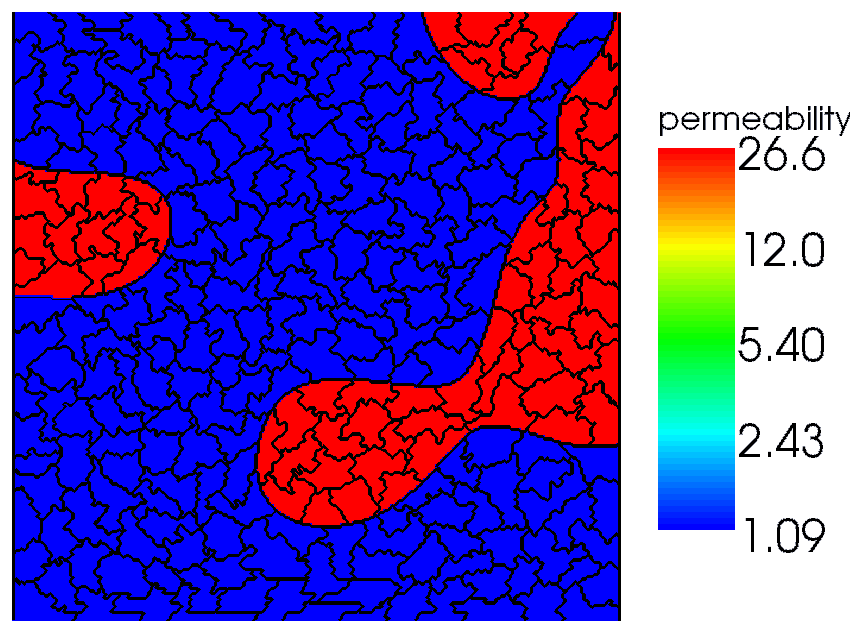
\includegraphics[width=.4\textwidth]{EPS/aggregates_problem_f_2d_65536_cl015_var8_mean0}
  \end{center}

    \begin{itemize}
    \item $-\nabla \cdot (k(x) \nabla u) = f \text{ in }\Omega$
    \item $\kappa (x)$ realization of log-random field with variance
      $\sigma^2$, mean $0$, and correlation length $\lambda$.
    \item $k(x)$: binary medium constructed from $\kappa (x)$.
    \item Weak scaling: $\lambda$ scales with mesh width $h$.
    \end{itemize}
  \end{frame}
\begin{frame}[fragile]
  \frametitle{Weak Scalability Results (Possion vs. Clipped)}
  \begin{center}
      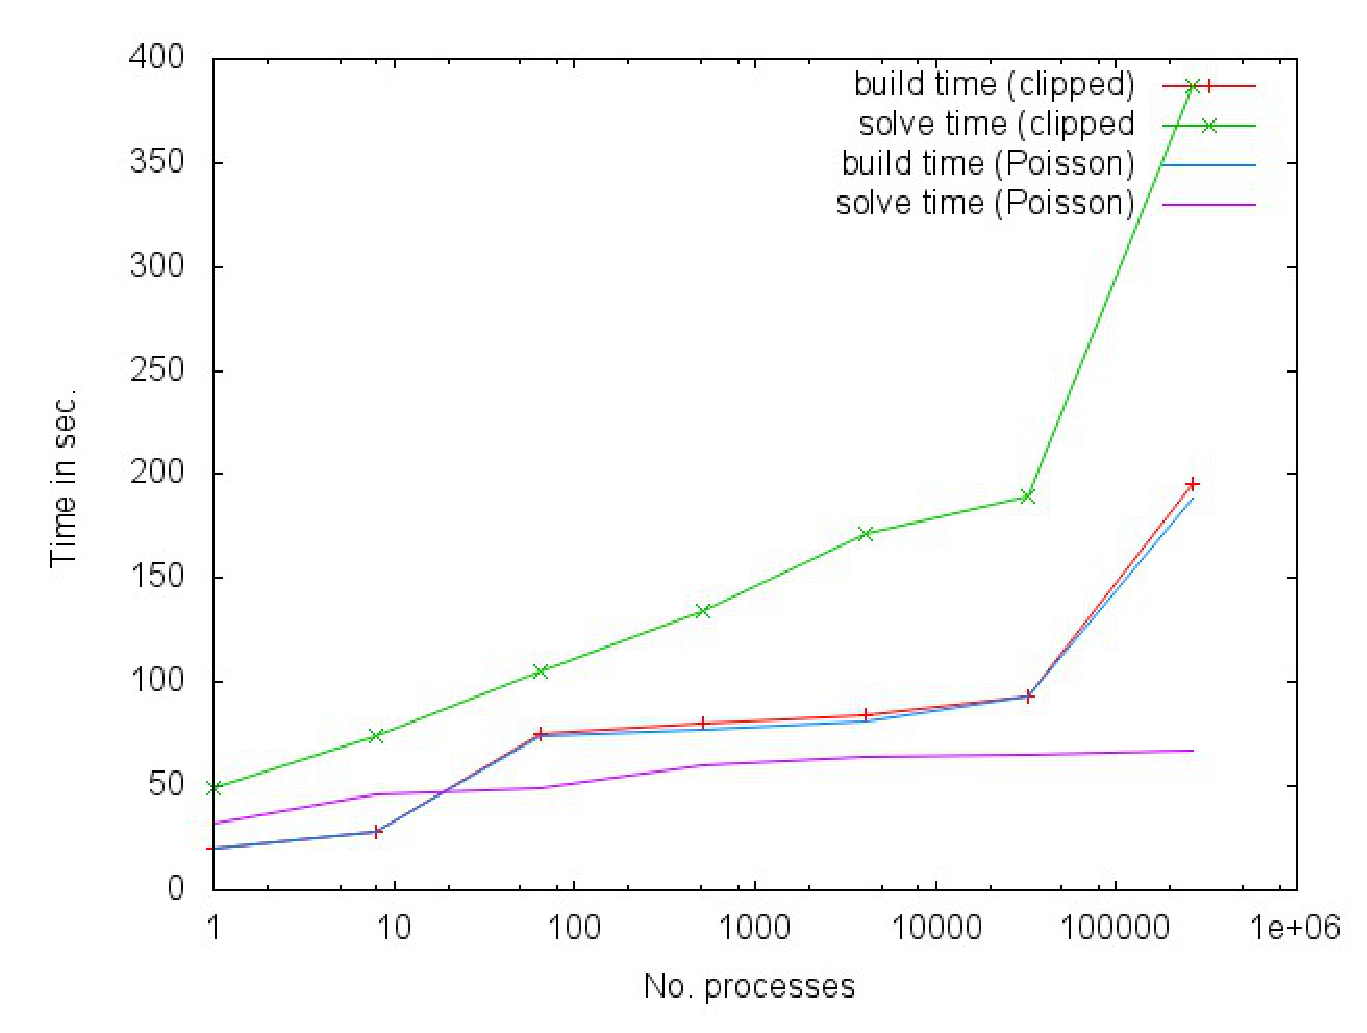
\includegraphics[width=.6\textwidth]{EPS/solve_build}
  \end{center}
  \begin{itemize}
  \item BiCGStab precondition with parallel AMG
  \item $1.34\cdot 10^{11}$ unknowns.
  \item Machine: IBM Blue Gene/P in J\"ulich with 294,849 cores
  \end{itemize}
\end{frame}
\subsection{PDELab Backends}
\label{sec:pdelab-backends-1}


\begin{frame}
  \frametitle<presentation>{PDELab backend}
  \begin{itemize}
  \item Linear algebra is decoupled from the discretization.
  \item Provides unique access interface for matrices, vectors and
    solvers.
  \item (Often) easily extensible for use of other libraries.
  \item Minimal knowledge of the underlying libraries required.
  \end{itemize}
\end{frame}

\begin{frame}
  \frametitle{PDELab backend in UML}
  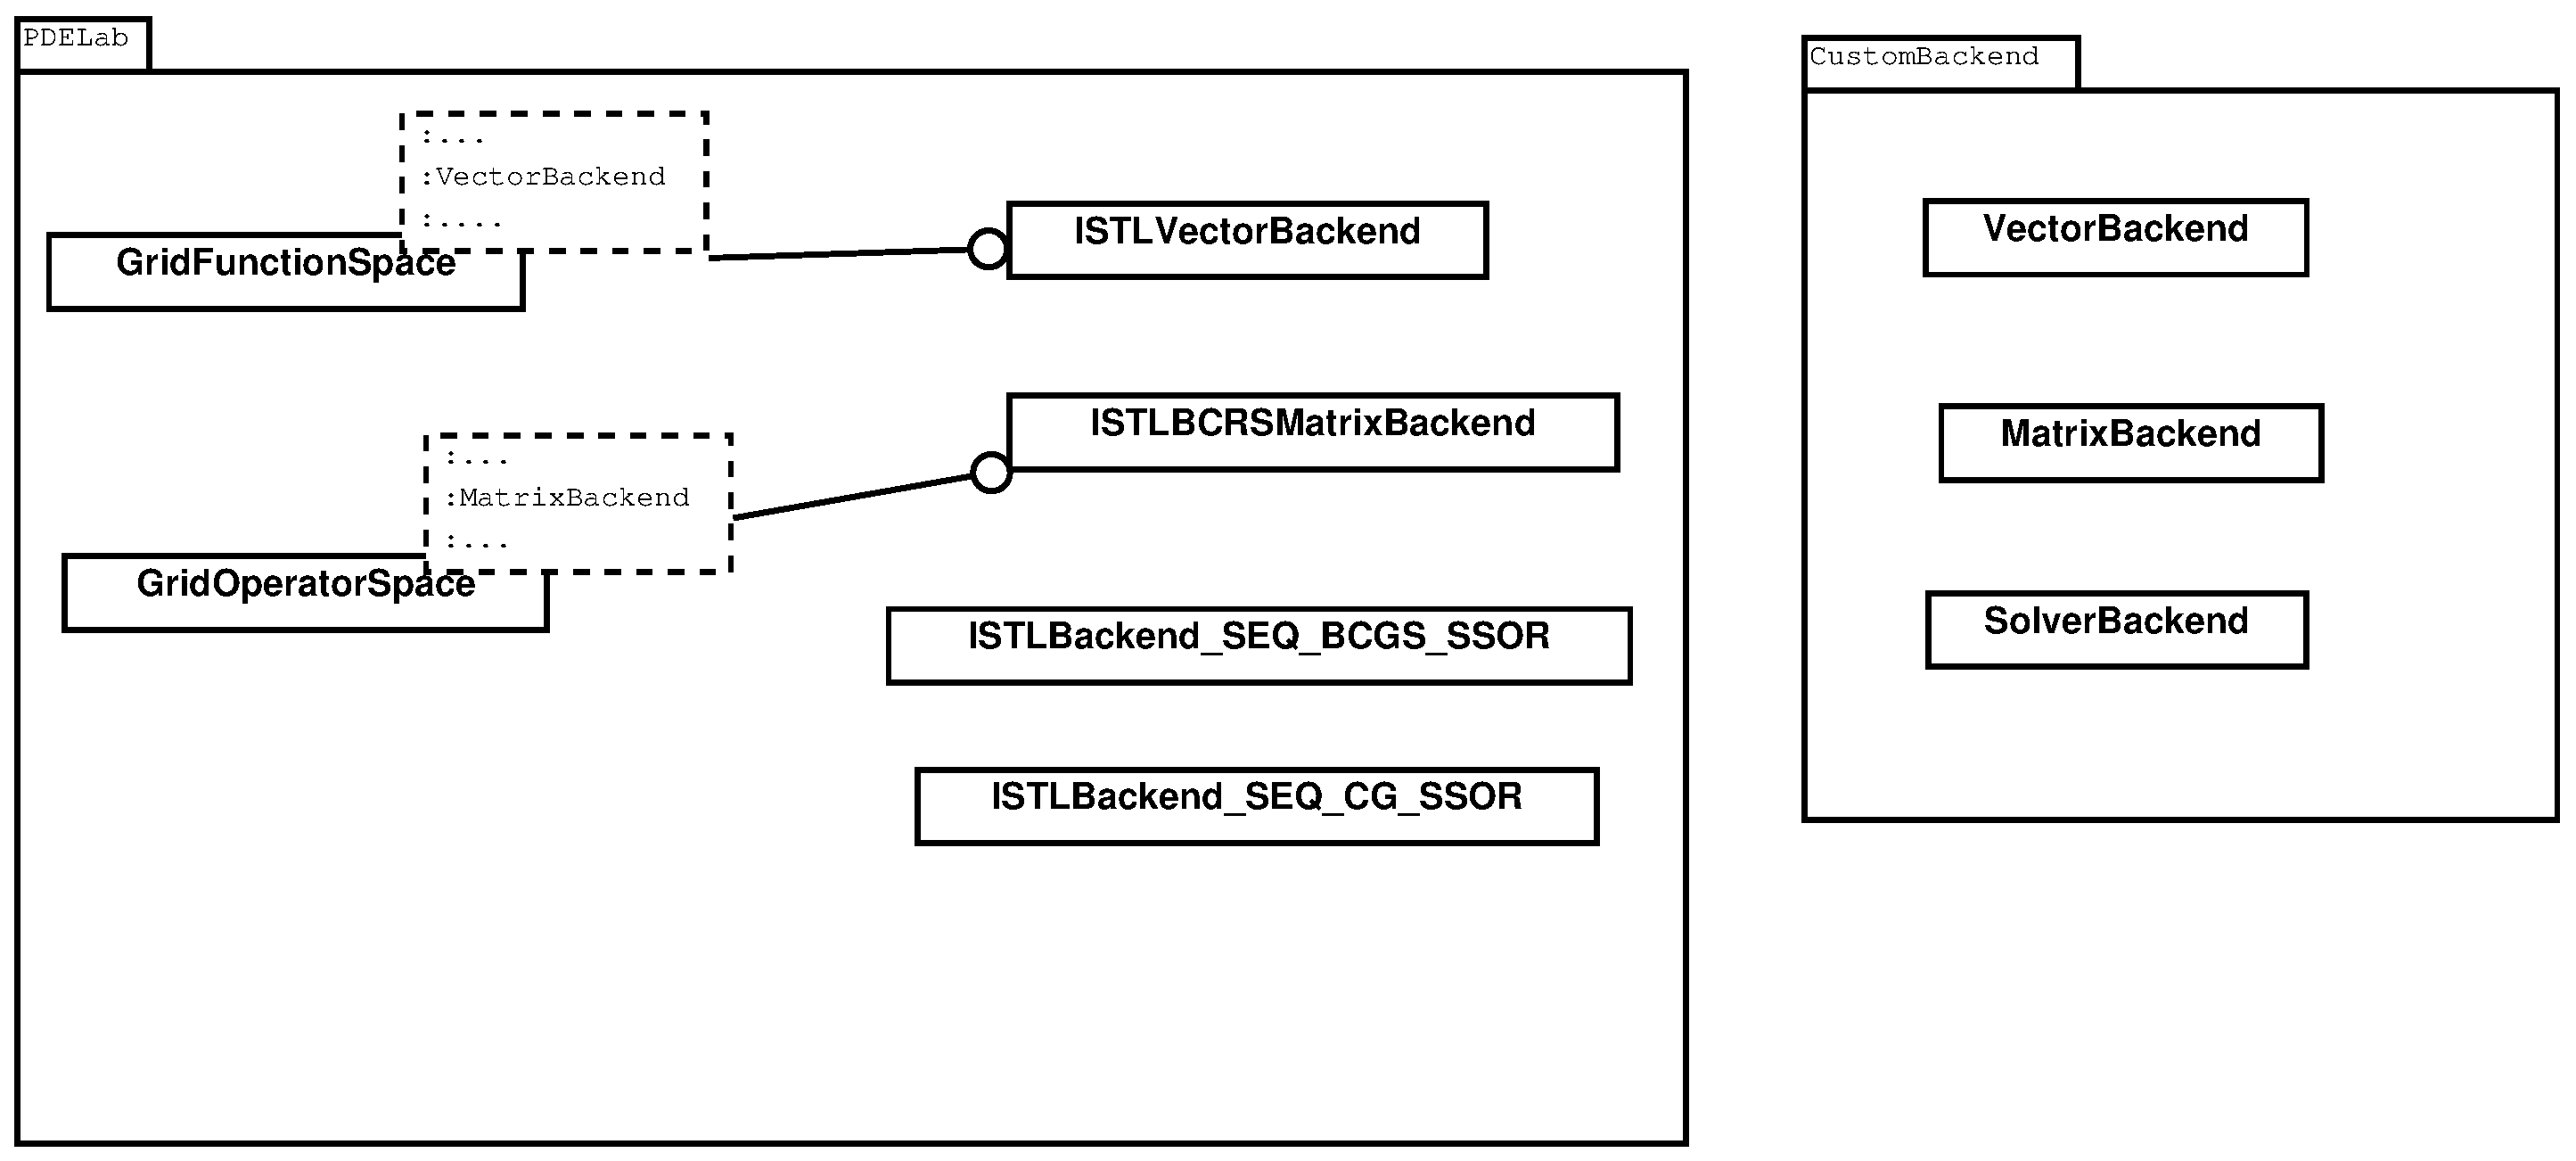
\includegraphics[width=\textwidth]{./EPS/backend}
\end{frame}

\subsubsection{The Vector Backend}
\label{sec:vector-backend}

\begin{frame}
  \frametitle<presentation>{The Vector Backend}
  \begin{itemize}
  \item It is a class not a namespace to allow template parameterization!
  \item Provides the actual container type as
    \lstinline!template<class T, class E> Vector!.
  \item Associated type \lstinline!size_type! used for index access.
  \item Const and mutable data access with
    \lstinline!access(Vector<T,E>& cont, size_type i)!
  \end{itemize}
\end{frame}

\begin{frame}[fragile]
  \frametitle{Sample Vector Container}
  \begin{itemize}
  \item Template parameter T is the type of the grid function used.
  \item Template parameter E is the value type (e.g. double, float).
  \end{itemize}
  \begin{lstlisting}[basicstyle=\scriptsize]
    template<typename T, typename E>
    class VectorContainer
    {
      public:
      // The stored element type
      typedef E ElementType;
      // The backend we are associated with
      typedef ISTLVectorBackend<BLOCKSIZE> Backend;

      //constructor with grid function space t
      VectorContainer (const T& t_);

      //constructor with grid function space t, initial value e
      VectorContainer (const T& t_, const E& e);

      // assignment
      VectorContainer& operator= (const E& e);
    };
  \end{lstlisting}
\end{frame}
\subsubsection{The Matrix Backend}
\label{sec:matrix-backend}

\begin{frame}
  \frametitle<presentation>{The Matrix Backend}
  \begin{itemize}
  \item It is a class not a namespace to allow template
    parameterization!
  \item Provides the actual container type as
    \lstinline!template<class T, class E> Matrix!.
%  \item Provides associated type \lstinline!Pattern! for setting up
%    the sparsity pattern.
  \item Provides method \lstinline!clearRow(RI i, C& c)! for setting
    the values of row with index $i$ of container \lstinline!c! to
    zero.
    \item Const and mutable data access with
    \lstinline!access(Matrix<T,E>& cont, size_type i, size_type j)!
  \end{itemize}
\end{frame}

\begin{frame}[fragile]
  \frametitle{The Matrix Container}
\begin{itemize}
  \item Template parameter T is the type of the grid function used.
  \item Template parameter E is the value type (e.g. double, float).
  \end{itemize}
  \begin{lstlisting}[basicstyle=\scriptsize]
template<class T, class E>
class MatrixContainer{
  public:
    // The stored element type
    typedef typename E ElementType;
    // The backend we are associated with
    typedef ISTLMatrixBackend<ROWBLOCKSIZE,COLBLOCKSIZE> Backend;

    //constructor with grid operator t
    // Needs to setup the whole sparsity pattern.
    MatrixContainer (const T& t_);

    // assignment
    MatrixContainer& operator= (const E& e);
};
  \end{lstlisting}
\end{frame}
\begin{frame}[fragile]
  \frametitle{Sparse Matrix Setup in PDELab}
  \begin{itemize}
  \item Setting up a sparse matrix is a two step procedure:
    \begin{enumerate}
    \item Setting up the sparsity pattern.
    \item Filling the matrix with the values.
    \end{enumerate}
  \item First step is performed by the contructor of the matrix
    container.
  \item Second step is performed by the member function
    \lstinline!jacobian! of the grid operator.
  \end{itemize}

\end{frame}

\subsubsection{The Linear Solver Backend}
\label{sec:line-solv-back}

\begin{frame}[fragile]
  \frametitle<presentation>{The Linear Solver Backend}
  \begin{itemize}
  \item Provides vector norm method needed by nonlinear PDELab solvers:
      \begin{lstlisting}
template<class V>
typename V::ElementType norm(const V& v) const;
      \end{lstlisting}
    \item Member function \lstinline!result()! returns statistics
      about the solution phase in an instance of the
      \lstinline!template<class T> LinearSolverResult! class template.
\item Use member function
  \begin{lstlisting}
template<class M.class V,class W>
apply(M& A, V& z, W& r, typename V::ElementType reduction);
  \end{lstlisting}
  to (iteratively) solve $Az=r$ until the prescribed relative defect
  reduction is achieved.
  \item For ISTL it hides a lot of the compexity that heavy usage of
    templates imposes on the user.
  \end{itemize}
\end{frame}

\subsubsection{The Backend}
\label{sec:backend}

\begin{frame}
  \frametitle{ISTL Vector Backend}
  \begin{itemize}
  \item \lstinline!template<int blocksize> class ISTLVectorBackend!
    is the currently available backend for ISTL vectors.
  \item The backend uses
    \lstinline!BlockVector<FieldVector<E,blocksize> >! as the
    underlying container.
  \item Attention: Make sure everything is correct for nonscalar backends
    \lstinline!blocksize!$>1$
  \end{itemize}
\end{frame}

\begin{frame}
  \frametitle{ISTL Matrix Backend}
  \begin{itemize}
    \item \lstinline!template<int brows,int bcols> class ISTLBCRSMatrixBackend!
      is the currently available backend for ISTL sparse
      matrices.
    \item \lstinline!brows! is the number of rows and \lstinline!bcols!
      is the number of columns of each matrix block.
  \item The backend uses
    \lstinline!BCRSMatrix<FieldMatrix<E,brows,bcols> >! as the
    underlying container.
  \item Attention: Make sure everything is correct for nonscalar backends
    \lstinline!blocksize!$>1$.
  \end{itemize}
\end{frame}
\begin{frame}[fragile]
  \frametitle{ISTL Sequential Solver Backends}
    \begin{itemize}
    \item \lstinline!ISTLBackend_SEQ_CG_SSOR!:  conjugate gradient method with SSOR preconditioner
    \item \lstinline!ISTLBackend_SEQ_BCGS_SSOR!: stabilized bi-conjugate gradient
      method with SSOR preconditioner
    \item \lstinline!ISTLBackend_SEQ_SuperLU!: SuperLU, a sparse
      direct solver
    \item \lstinline!template<class T> class ISTLBackend_SEQ_CG_AMG_SSOR! and
      \lstinline!template<class T> class ISTLBackend_SEQ_BCGS_AMG_SSOR!
      use a point-block AMG based on aggregation smoothed by SSOR as
      the preconditioner
    \end{itemize}
    Currently these sequential solvers are just a subset of the ones
  available in ISTL directly. More will follow in due time.
\end{frame}

\begin{frame}[fragile]
  \frametitle{Putting it all together}
  \scriptsize
  \begin{lstlisting}
  // make grid function space
  typedef Dune::PDELab::NoConstraints CON;
  typedef Dune::PDELab::ISTLVectorBackend
    <Dune::PDELab::ISTLParameters::static_blocking,blocksize> VBE;
  typedef Dune::PDELab::GridFunctionSpace<GV,FEM,CON,VBE> GFS;
  GFS gfs(gv,fem);

  // make local operator
  Dune::PDELab::ConvectionDiffusionDGMethod::Type m
    = Dune::PDELab::ConvectionDiffusionDGMethod::SIPG;
  Dune::PDELab::ConvectionDiffusionDGWeights::Type w
    = Dune::PDELab::ConvectionDiffusionDGWeights::weightsOn;
  typedef Dune::PDELab::ConvectionDiffusionDG<PROBLEM,FEM> LOP;
  LOP lop(problem,m,w,alpha);
  typedef Dune::PDELab::ISTLMatrixBackend MBE;
  typedef typename GFS::template ConstraintsContainer<Real>::Type CC;
  CC cc;
  typedef Dune::PDELab::GridOperator<GFS,GFS,LOP,MBE,Real,Real,Real,CC,CC> GO;
  GO go(gfs,cc,gfs,cc,lop);
  typedef Dune::PDELab::ISTLBackend_SEQ_CG_ILU0 LS;
  LS ls(10000,1);
  typedef Dune::PDELab::StationaryLinearProblemSolver<GO,LS,U> SLP;
  SLP slp(go,u,ls,1e-12);
  slp.apply();
  \end{lstlisting}
\end{frame}
% \subsection{Parallel PDELab}
% \label{sec:parallelization}

% \begin{frame}
%   \frametitle<presentation>{Parallel PDELab}
%   \begin{itemize}
%   \item Go parallel by choosing
%     \begin{enumerate}
%     \item a suitable parallel grid (e.g. an overlapping one for
%       overlapping domain decomposition methods),
%     \item the correct constraints for the discretization of
%       the PDE, and
%     \item a suitable and matching parallel solver backend of the
%       PDELab backend.
%     \end{enumerate}
%   \end{itemize}
% \end{frame}

% \begin{frame}
%   \frametitle<presentation>{Parallel Solver Backends}

%   There are three different kinds of parallel solvers classes
%   available in the ISTL backend:
%   \begin{itemize}
%   \item Nonoverlapping domain decomposition
%     methods.
%   \item Overlapping domain decomposition metods.
%   \item Data parallel solvers (e.g. AMG).
%   \end{itemize}
% \end{frame}

% \begin{frame}
%   \frametitle<presentation>{Building Blocks for Parallel Solvers}
%   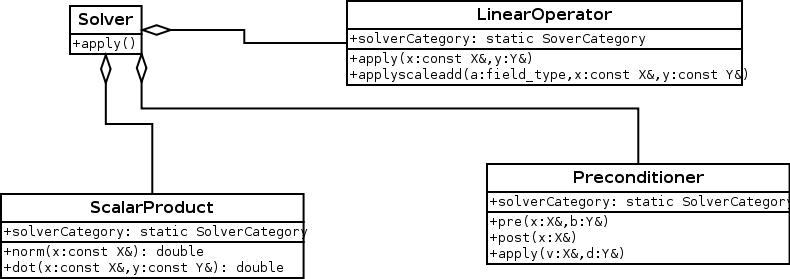
\includegraphics[width=\textwidth]{EPS/istlsolver}
% \end{frame}

% \begin{frame}
%   \frametitle{Some Parallel Solver Backends}
%   The solver backends can be found in header
%   dune/pdelab/backend/istlsolverbackend.hh. Template parameter GFS is
%   the type of the grid function space, template parameter C the type
%   of the parallel constraints used.
%   \begin{itemize}
%   \item \lstinline!template<class GFS> class ISTLBackend_NOVLP_BCGS_NOPREC!:
%     parallel unpreconditioned
%     stabilized bi-conjugate gradient method for nonoverlapping grids.
%     \item \lstinline!template<class GFS> class ISTLBackend_OVLP_BCGS_SSORk!:
%       the above preconditioned with $k$ steps of SSOR.
%     \item \lstinline!template<class GFS, class C> class ISTLBackend_OVLP_BCGS_SuperLU!:
%       the first method preconditioned by an overlapping domain
%       decomposition method with SuperLU for the problems local to the
%       processors.
%       \item \lstinline!template<class GFS> ISTLBackend_BCGS_AMG_SSOR!:
%         the first method preconsitioned by parallel AMG smoothed by
%         SSOR. Requires an overlapping grid!
%   \end{itemize}
% \end{frame}

% \begin{frame}[fragile]
%   \frametitle{Nonoverlapping example}
%   \begin{lstlisting}[basicstyle=\tiny]
% // 1. Create an non-overlapping grid
% Dune::FieldVector<double,2> L(1.0);
% Dune::FieldVector<int,2> N(16);
% Dune::FieldVector<bool,2> periodic(false);
% int overlap=0; // needs overlap 0 because overlap elements are not assembled
% Dune::YaspGrid<2> grid(helper.getCommunicator(),L,N,periodic,overlap);
% typedef Dune::YaspGrid<2>::LeafGridView GV;
% const GV& gv=grid.leafView();

% // 2. Create correctly constrained grid function space
% typedef Dune::PDELab::Q1LocalFiniteElementMap<Coord,Real,dim> FEM;
% FEM fem;
% typedef Dune::PDELab::NonoverlappingConformingDirichletConstraints CON;
% CON con;
% typedef Dune::PDELab::ISTLVectorBackend<1> VBE;
% typedef Dune::PDELab::GridFunctionSpace<GV,FEM,CON,VBE,
% Dune::PDELab::SimpleGridFunctionStaticSize> GFS;
% GFS gfs(gv,fem,con);
% con.compute_ghosts(gfs); // con stores indices of ghost dofs
% typedef ConvectionDiffusionProblem<GV,Real> Param;
% Param param;
% typedef Dune::PDELab::BoundaryConditionType_CD<Param> B;
% B b(gv,param);
% typedef Dune::PDELab::DirichletBoundaryCondition_CD<Param> G;
% G g(gv,param);
% \end{lstlisting}
% \end{frame}
% \begin{frame}[fragile]
% \frametitle<presentation>{Nonoverlapping Example Continued}
%   \begin{lstlisting}[basicstyle=\tiny]
% // Compute constrained space
% typedef typename GFS::template ConstraintsContainer<Real>::Type C;
% C cg;
% Dune::PDELab::constraints(b,gfs,cg);

% // Compute affine shift
% typedef typename GFS::template VectorContainer<Real>::Type V;
% V x(gfs,0.0);
% Dune::PDELab::interpolate(g,gfs,x);
% Dune::PDELab::set_nonconstrained_dofs(cg,0.0,x);

% // Make grid operator space
% typedef Dune::PDELab::ConvectionDiffusion<Param> LOP;
% LOP lop(param,2);
% typedef Dune::PDELab::ISTLBCRSMatrixBackend<1,1> MBE;
% typedef Dune::PDELab::GridOperatorSpace<GFS,GFS,LOP,C,C,MBE,true> GOS;
% GOS gos(gfs,cg,gfs,cg,lop);

% // 3. Choose a linear solver
% typedef Dune::PDELab::ISTLBackend_NOVLP_BCGS_NOPREC<GFS> LS;
% LS ls(gfs,5000,1);
% ...
% \end{lstlisting}

% \end{frame}

% \begin{frame}[fragile]
%   \frametitle{Overlapping Example}
%   \begin{lstlisting}[basicstyle=\tiny]
% // 1. Create an overlapping grid
% Dune::FieldVector<double,2> L(1.0);
% Dune::FieldVector<int,2> N(16);
% Dune::FieldVector<bool,2> periodic(false);
% int overlap=2;
% Dune::YaspGrid<2> grid(helper.getCommunicator(),L,N,periodic,overlap);
% typedef Dune::YaspGrid<2>::LeafGridView GV;
% const GV& gv=grid.leafView();

% // 2. Create correctly constrained grid function space
% typedef Dune::PDELab::Q1LocalFiniteElementMap<Coord,Real,dim> FEM;
% FEM fem;
% typedef Dune::PDELab::OverlappingConformingDirichletConstraints CON;
% typedef Dune::PDELab::ISTLVectorBackend<1> VBE;
% typedef Dune::PDELab::GridFunctionSpace<GV,FEM,CON,VBE,
% Dune::PDELab::SimpleGridFunctionStaticSize> GFS;
% GFS gfs(gv,fem);

% //  define problem parameters
% typedef ConvectionDiffusionProblem<GV,Real> Param;
% Param param;
% typedef Dune::PDELab::BoundaryConditionType_CD<Param> B;
% B b(gv,param);
% typedef Dune::PDELab::DirichletBoundaryCondition_CD<Param> G;
% G g(gv,param);
% \end{lstlisting}
% \end{frame}
% \begin{frame}[fragile]
% \frametitle<presentation>{Overlapping Example Continued}
%   \begin{lstlisting}[basicstyle=\tiny]

% //  Compute constrained space
% typedef typename GFS::template ConstraintsContainer<Real>::Type C;
% C cg;
% Dune::PDELab::constraints(b,gfs,cg);
% //  Compute affine shift
% typedef typename GFS::template VectorContainer<Real>::Type V;
% V x(gfs,0.0);
% Dune::PDELab::interpolate(g,gfs,x);
% Dune::PDELab::set_nonconstrained_dofs(cg,0.0,x);
% // Make grid operator space
% typedef Dune::PDELab::ConvectionDiffusion<Param> LOP;
% LOP lop(param,2);
% typedef Dune::PDELab::ISTLBCRSMatrixBackend<1,1> MBE;
% typedef Dune::PDELab::GridOperatorSpace<GFS,GFS,LOP,C,C,MBE> GOS;
% GOS gos(gfs,cg,gfs,cg,lop);

% // 3. Choose a linear solver
% typedef Dune::PDELab::ISTLBackend_OVLP_BCGS_SuperLU<GFS,C> LS;
% LS ls(gfs,cg,5000,2);
% ...
% \end{lstlisting}

% \end{frame}
%\lstset{breakatwhitespace=false,breaklines=false}

\cleardoublepage

%%% Local Variables:
%%% mode: latex
%%% TeX-master:
%%% End:
